\documentclass[tikz,border=8pt]{standalone}
% Shared look for every TikZ diagram. Load with \input{../../tools/tikz-style.tex}
\usepackage[T1]{fontenc}
\usepackage{lmodern}
\renewcommand{\sfdefault}{lmr}  % diagrams use the same serif as the text
\usetikzlibrary{arrows.meta, positioning, shapes.geometric, calc, fit, backgrounds}
\definecolor{cblue}{HTML}{4C78A8}
\definecolor{corange}{HTML}{F58518}
\definecolor{cgreen}{HTML}{54A24B}
\definecolor{cred}{HTML}{E45756}
\definecolor{cpurple}{HTML}{B279A2}
\definecolor{cgrey}{HTML}{6B6B6B}
\tikzset{
  every picture/.style={font=\sffamily, line width=1.2pt},
  box/.style={draw=#1, fill=#1!12, rounded corners=4pt, align=center, inner sep=7pt, minimum height=1.1cm},
  box/.default=cgrey,
  arrow/.style={-{Stealth[length=3mm]}, draw=cgrey, line width=1.4pt},
  title/.style={font=\sffamily\bfseries\Large},
  note/.style={font=\sffamily\small, text=cgrey, align=center},
}
\AtBeginDocument{\hyphenpenalty=10000 \exhyphenpenalty=10000}

\begin{document}
\begin{tikzpicture}[b/.style={box=cblue, minimum width=4.6cm}, g/.style={box=cgrey, minimum width=4.6cm},
  o/.style={box=corange, minimum width=4.6cm}]
  \node[g] (w) at (0,0) {1. every row gets weight $1/n$};
  \node[b] (fit) at (0,-1.7) {2. fit a decision stump};
  \node[o] (err) at (0,-3.4) {3. error = sum of the weights\\of the misclassified rows};
  \node[o] (a) at (0,-5.3) {4. say: $\alpha = \dfrac{1}{2}\ln \dfrac{1-\text{error}}{\text{error}}$};
  \node[g] (up) at (7,-5.3) {5. update the weights:\\mistakes $\times e^{\alpha}$, correct $\times e^{-\alpha}$};
  \node[g] (norm) at (7,-3.4) {6. normalise: divide by the sum};
  \node[g] (res) at (7,-1.7) {7. upsample: draw $n$ rows\\with these weights};
  \node[g] (new) at (7,0) {new dataset for the next stage};
  \draw[arrow] (w) -- (fit); \draw[arrow] (fit) -- (err); \draw[arrow] (err) -- (a);
  \draw[arrow] (a) -- (up); \draw[arrow] (up) -- (norm); \draw[arrow] (norm) -- (res); \draw[arrow] (res) -- (new);
  \draw[arrow, dashed] (new) -- node[note, above] {repeat} (w);
\end{tikzpicture}
\end{document}
